% ----------------------------------------------------------
\section{Calibração dos sistemas de baixo custo para monitoramento da qualidade do ar}\label{section:monit-low-cost-calib}
% ----------------------------------------------------------

A calibração implica na obtenção de um modelo matemático que converta o parâmetro medido (e.g. adsorção de luz, tensão, condutividade, corrente elétrica, etc) na variável de saída desejada (e.g. concentração do poluente). Na maioria dos casos, os sensores de gases já possuem uma calibração de fábrica. Inclusive, sensores digitais como os do fabricante SPEC Sensors, já são disponibilizados com um \textit{software} embarcado que entrega as leituras de concentração calibradas e compensadas pelos efeitos da temperatura e a umidade relativa \cite{SPECSensors2017Digital968-045}. Outros fabricantes, como Alphasense, disponibilizam constantes de calibração e modelos lineares de compensação que podem ser aplicados à saída dos sensores para obter as leituras de concentração \cite{Alphasense2019AlphasenseSensors}.

Os modelos e parâmetros disponibilizados nos manuais de usuário, folhas técnicas e notas de aplicação dos sensores de gases são obtidos através de testes de laboratório realizados pelo próprio fabricante em condições controladas. Por isso, quando testados pelo usuário da tecnologia em condições laboratoriais semelhantes, o desempenho dos dispositivos costuma ser favorável. Contudo, as informações providas por estes meios são insuficientes para o amplo e diverso espectro de condições de operação dos sensores \cite{Morawska2018ApplicationsGone}. Por este motivo, a literatura recomenda a execução de rotinas de testes e calibração que comprovem o comportamento dos sensores e determinem sua aptidão para a aplicação em que serão utilizados \cite{Williams2014AirGuidebook,Lewis2018Low-costApplications}. 

As rotinas de calibração dos sensores em condições de laboratório possibilitam detectar e eliminar fontes de erro internas relacionadas com a fabricação e princípio de funcionamento dos dispositivos, como por exemplo: limites dinâmicos, erros sistemáticos de offset e sensibilidade e não linearidades \cite{Spinelle2013ProtocolPollution}. Nestas rotinas os sensores são expostos a diferentes níveis de concentração dentro de uma câmara de medição que tem acoplado um sistema de diluição e instrumentos de referência para medição de gases. Nesta câmara são gerados, dentro dos intervalos de interesse, cenários artificiais que representem as condições médias de temperatura, umidade relativa, pressão e níveis de concentração de poluentes onde se espera que o sensor será utilizado no longo prazo \cite{Spinelle2013ProtocolPollution}.
Porém, é consenso na literatura que estas calibrações não são suficiente para validar o desempenho dos sensores em aplicações reais, já que são incapazes de abranger a totalidade de condições operacionais possíveis \cite{Maag2018ADeployments,Lewis2018Low-costApplications,Morawska2018ApplicationsGone}. A presença e as variações não controladas de múltiplas espécies gasosas e das condições atmosféricas fazem necessária uma segunda etapa de calibração, em campo, que produza resultados mais consistentes com a realidade da aplicação.

As rotinas de calibração em campo possibilitam avaliar o comportamento dos dispositivos de baixo custo em condições que melhor se aproximem do cenário de aplicação de longo prazo. Nelas, os sensores são colocados junto a estações de referência previamente calibrados e validados por agências reguladoras. Para cobrir as diversas condições atmosféricas, a sazonalidade, e a gama de valores de concentração dos gases de interesse e dos gases interferentes, a literatura recomenda uma duração mínima de três meses para a execução das rotinas de calibração e dos testes de validação \cite{Spinelle2013ProtocolPollution}. Todavia, tem sido comprovado que sensores calibrados e testados com bom desempenho em determinado local, não reproduzem os mesmos resultados em outras localidades \cite{Zimmerman2018AMonitoring,Hagan2018CalibrationInstruments,Concas2019ACalibration}.

Vários fatores ocasionam isso. Um deles está dado pela distribuição log-normal que caracteriza às leituras de concentração, o que dificulta a aquisição de amostras de concentração elevada, em quantidades representativas para treinar os modelos de calibração. Isso ocasiona que as medições dos sensores produzam erros não desprezíveis quando expostos a ambientes com concentrações de poluentes maiores do que as encontradas durante o treinamento do modelo \cite{Zimmerman2018AMonitoring}. 
Igualmente, a variação das condições atmosféricas, dos níveis de concentração de poluentes e das fontes de emissão de um local para outro, dificulta a aplicação de um mesmo modelo de calibração em locais diferentes, por exemplo: ambientes urbanos vs. ambientes rurais, áreas residenciais vs. áreas com movimento intenso de veículos, ou áreas com predominância de fontes industriais vs. fontes naturais \cite{Hagan2018CalibrationInstruments,Zimmerman2018AMonitoring}.

A literatura reporta várias técnicas de calibração e de compensação que têm sido aplicadas nos sensores de baixo custo para o monitoramento da qualidade do ar com resultados promissores. De forma geral, os modelos de calibração utilizados podem ser agrupados em: modelos paramétricos univariados, modelos paramétricos multivariados e modelos multivariados não-paramétricos. Outros autores também têm aplicado algoritmos de compensação que removem os efeitos da temperatura e da umidade relativa das respostas dos sensores. 

A regressão univariada é a técnica de calibração paramétrica mais básica reportada na literatura. Esses modelos de calibração ajustam o sinal de saída do sensor (corrente, tensão, resistência elétrica, etc.) para seguir uma curva com valores de concentração de referência, sem considerar a interferência de outras variáveis como a temperatura, a umidade relativa e as sensibilidades cruzadas \cite{Maag2018ADeployments}. Estes modelos caracterizam-se por produzir os piores resultados em termos de erro e incerteza das medições em campo.

A regressão linear multivariada é uma regressão linear de múltiplas variáveis. Pelo fato de considerarem outras variáveis além das leituras de um só sensor, este modelo de regressão produz melhores resultados do que a regressão univariada \cite{Karagulian2019ReviewMonitoring}. No entanto, tem sido verificado que em concentrações na ordem dos \gls{ppb} estes modelos não são capazes de produzir resultados satisfatórios já que, nesta gama de valores, a temperatura e a umidade relativa produzem não linearidades nas respostas dos sensores que o modelo linear é incapaz de reproduzir \cite{Hagan2018CalibrationInstruments}. Já em concentrações maiores seu desempenho costuma ser tão bom quanto os modelos de aprendizado de máquina, pois nestes intervalos prevalece a dinâmica linear entre concentração do gás e a saída do sensor \cite{Hagan2018CalibrationInstruments}. Estes modelos, por serem paramétricos, conseguem extrapolar, com erro baixo, novos valores fora do intervalo de treinamento. Isto é vantajoso pois valores altos de concentração são pouco frequentes durante o treinamento em campo, devido à distribuição log-normal que caracteriza as variáveis de concentração.

A regressão não paramétrica, baseada em técnicas de aprendizado de máquina, possibilita elaborar modelos de calibração, a partir de dados coletados, sem a necessidade de complexos modelos paramétricos não-lineares \cite{Maag2018ADeployments}. Estas técnicas têm se mostrado uma alternativa eficiente em termos de erro e incerteza, e a maioria deles conseguem resultados iguais ou melhores em comparação com o restante dos modelos de calibração \cite{Feng2019ReviewTechnology}. Especificamente nos intervalos de baixas concentrações os modelos de aprendizado de máquina são superiores aos paramétricos já que conseguem lidar com as não linearidades que afetam as leituras dos sensores nestes intervalos \cite{Malings2019DevelopmentMonitoring}. Contudo, estes modelos  são mais limitados em ambientes com concentração elevada de poluentes devido a dois fatores principais: (1) a limitação para extrapolar valores fora do intervalo de treinamento \cite{Hagan2018CalibrationInstruments} e (2) a distribuição log-normal que caracteriza às variáveis de concentração, limitando a quantidade de amostras de concentração elevada que podem ser utilizadas para treinamento \cite{Zimmerman2018AMonitoring}.

Uma alternativa que vem produzindo resultados favoráveis é a aplicação de modelos de calibração híbridos. Estes modelos combinam técnicas de aprendizado de máquina e regressões lineares multivariadas para calibrar os sensores em duas faixas de concentração: altas e baixas. Dessa forma, o modelo híbrido consegue aproveitar o bom desempenho das técnicas de aprendizado de máquina nas baixas concentrações e o dos modelos lineares multivariados nas altas. Dois trabalhos têm reportado a aplicação desta alternativa e em ambos os resultados foram satisfatórios, já que os autores conseguiram reduzir a influência da temperatura e a umidade nas medições assim como reutilizar o mesmo modelo de calibração em diferentes locais com uma boa correlação e baixos valores de erro e incerteza \cite{Hagan2018CalibrationInstruments,Malings2019DevelopmentMonitoring}.

Dada a variedade de técnicas de aprendizado de máquina, é interessante comparar o desempenho daquelas que já tem sido utilizadas em modelos de calibração híbridos, i.e.: regressão pelos k-vizinhos mais próximos \cite{Hagan2018CalibrationInstruments} e as florestas aleatórias \cite{Malings2019DevelopmentMonitoring}. Um algoritmo de aprendizado de máquina bem popular \cite{Feng2019ReviewTechnology} dentre os modelos de calibração de monitores de baixo custo é a regressão por redes neurais artificiais \cite{Concas2019ACalibration}. Como os modelos híbridos ainda são bem incipientes é interessante comparar o desempenho dessas três técnicas de \gls{ml} dentro de um modelo híbrido. Também, pela robustez que os modelos híbridos têm demonstrado sob condições ambientais variadas, resulta interessante testar seu desempenho em aplicações de monitoramento móvel. Até o momento, não se tem conhecimento de estudos que tenham sido realizados nessa direção.

% ----------------------------------------------------------
\subsection{Redes Neurais Artificiais}
% ----------------------------------------------------------

As redes neurais artificiais (\gls{ann}) são sistemas de processamento paralelo inspirados nos neurônios biológicos. Uma das topologias mais populares de redes neurais é a Perceptron multicamadas (Figura \ref{fig:monit-calib-mlp-structure}) \cite{geron2019maos}. A rede contém uma camada de entrada, que são as entradas do modelo; uma camada de saída e uma ou várias camadas ocultas. As camadas de saída e as ocultas estão compostas por neurônios artificiais que aplicam uma função de transferência sigmoidal sobre suas entradas \cite{Feng2019ReviewTechnology}. O objetivo da rede é predizer os valores de saída com o mínimo valor de erro. Para isso é aplicado um algoritmo de otimização que ajusta os pesos das funções de transferência dentro dos neurônios para minimizar o erro. O algoritmo de otimização mais conhecido é o de Retropropagação do Erro \cite{geron2019maos}.

\begin{figure}[h]
    \centering
    \caption{Perceptron Multicamadas}
    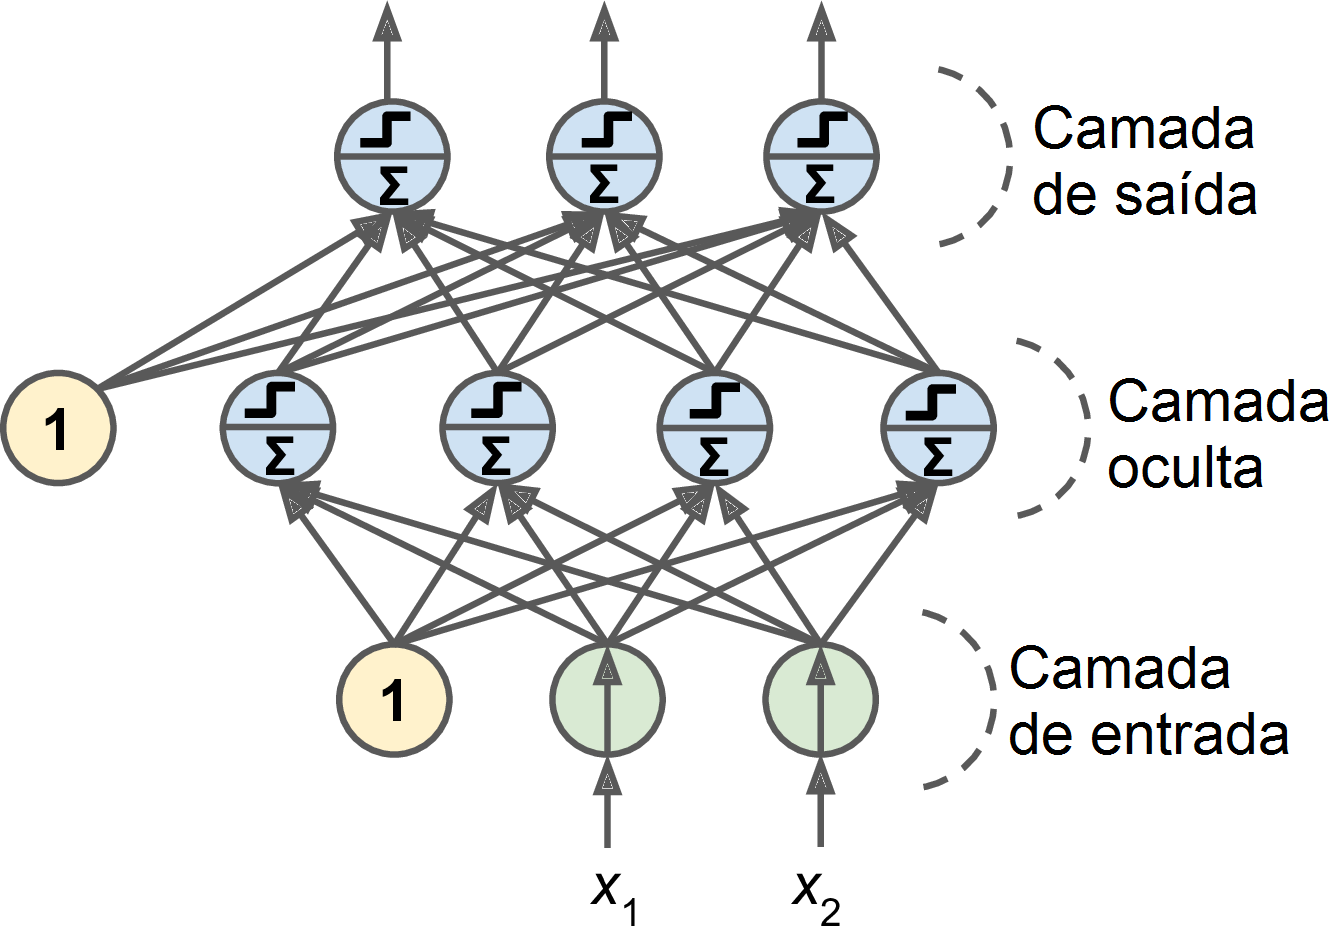
\includegraphics[width=0.5\textwidth]{chapters/1-MONITORAMENTO/Figuras/MLP_PT.png}
    \label{fig:monit-calib-mlp-structure}
    \fonte{\cite{geron2019maos}}
\end{figure}

As \gls{ann} têm sido muito usadas para problemas de predição e generalização já que conseguem modelar inúmeros sistemas. Especificamente nos sistemas de baixo custo para monitoramento de gases têm se mostrado uma solução eficaz \cite{Spinelle2015FieldDioxide,Spinelle2017FieldCO2,DeVito2018CalibratingApproaches}. Principalmente em intervalos baixos de concentração, esta alternativa supera aos modelos \gls{mlr}, pois consegue capturar melhor as não linearidades produzidas pela interferência de outras variáveis. Contudo, em intervalos de concentração elevados, seu desempenho cai já que estes modelos de aprendizado de máquina não conseguem extrapolar valores fora do intervalo de treinamento.

% ----------------------------------------------------------
\subsection{Florestas Aleatórias}
% ----------------------------------------------------------

A Floresta Aleatória é uma técnica de aprendizado supervisionado de máquinas. Uma floresta aleatória está constituida por um conjunto de árvores de decisão construídos a partir do conjunto de dados de treinamento \cite{geron2019maos}. O valor médio obtido do conjunto de árvores é depois usado para predizer novos dados de entrada. A idéia das florestas aleatórias é que a decisão de um conjunto de modelos medíocres é melhor que a de um único modelo bom. Isso também os torna menos propensos a sobre-ajustes.

Em comparação com as redes neurais, as florestas aleatórias precisam de um volume de dados menor e são menos intensas computacionalmente \cite{Montantes20203Science}. Vários trabalhos sobre monitoramento de gases de baixo custo têm aplicado modelos de calibração deste tipo com resultados satisfatórios, comparáveis aos obtidos com redes neurais \cite{Karagulian2019ReviewMonitoring}. Elas também têm como vantagem que seus resultados são interpretáveis.

% ----------------------------------------------------------
\subsection{K Vizinhos Mais Próximos}
% ----------------------------------------------------------

O método \gls{knn} baseia-se na suposição de que coisas semelhantes se encontram próximas. O algoritmo prediz o valor de determinada amostra de uma variável a partir dos valores das k amostras conhecidas mais próximas \cite{Altman1992AnRegression}. Para predizer o valor de uma amostra desconhecida, o algoritmo seleciona, dentro do conjunto de treinamento, as k amostras que se encontram mais próximas dela, considerando as variáveis de entrada do modelo. Logo, o algoritmo calcula o novo valor como a média dos valores de saída das amostras de treinamento \cite{Kramer2013K-NearestNeighbors}. Como medida para a distância entre as amostras costuma-se utilizar a distância euclidiana ou a distância Manhattan. O número de vizinhos é determinado mediante uma grade de busca durante o treinamento do modelo para garantir baixo erro na predição de amostras desconhecidas \cite{Miller2019TheScience}. Este algoritmo consegue modelar bem sistemas não-lineares e o tempo de treinamento é curto, porém o tempo de predição é longo e para conjuntos de dados muito extensos o tempo de processamento pode ser muito demorado. Outra desvantagem deste algoritmo é que seus resultados são difíceis de interpretar pois não é possível saber qual é o peso de cada variável dentro do modelo.

% ----------------------------------------------------------
\subsection{Redes de monitoramento de baixo custo}
% ----------------------------------------------------------

% ----------------------------------------------------------
\subsection{Lacunas científicas no monitoramento de baixo custo}
% ----------------------------------------------------------